\section{Laboratory work implementation}

\subsection{Tasks and Points}

\begin{enumerate}

\item Create an animation based on Windows timer which involves at least 5 different drawn objects
\item Increase and decrease animation speed using mouse wheel/from keebord

\end{enumerate}
\subsection{Laboratory work analysis}

Link to my GitHub repository : 

\url{https://github.com/Tolea86/WP_ANDROID/tree/master/LAB_4/PW_LAB4}\\

My application has following features : it has 1 view with 5 drawn objects in it and a button centered to the middle. Clicking on the button from center will make it disappear and will start the animation of the objects at the duration of 200 ms. Clicking on the screen will decrease the duration by 100 on every click. Clicking on back button from android will stop the animation at all, will make visible the center button and will reset duration to 200 ms.

\subsection{Prove your work with screens}

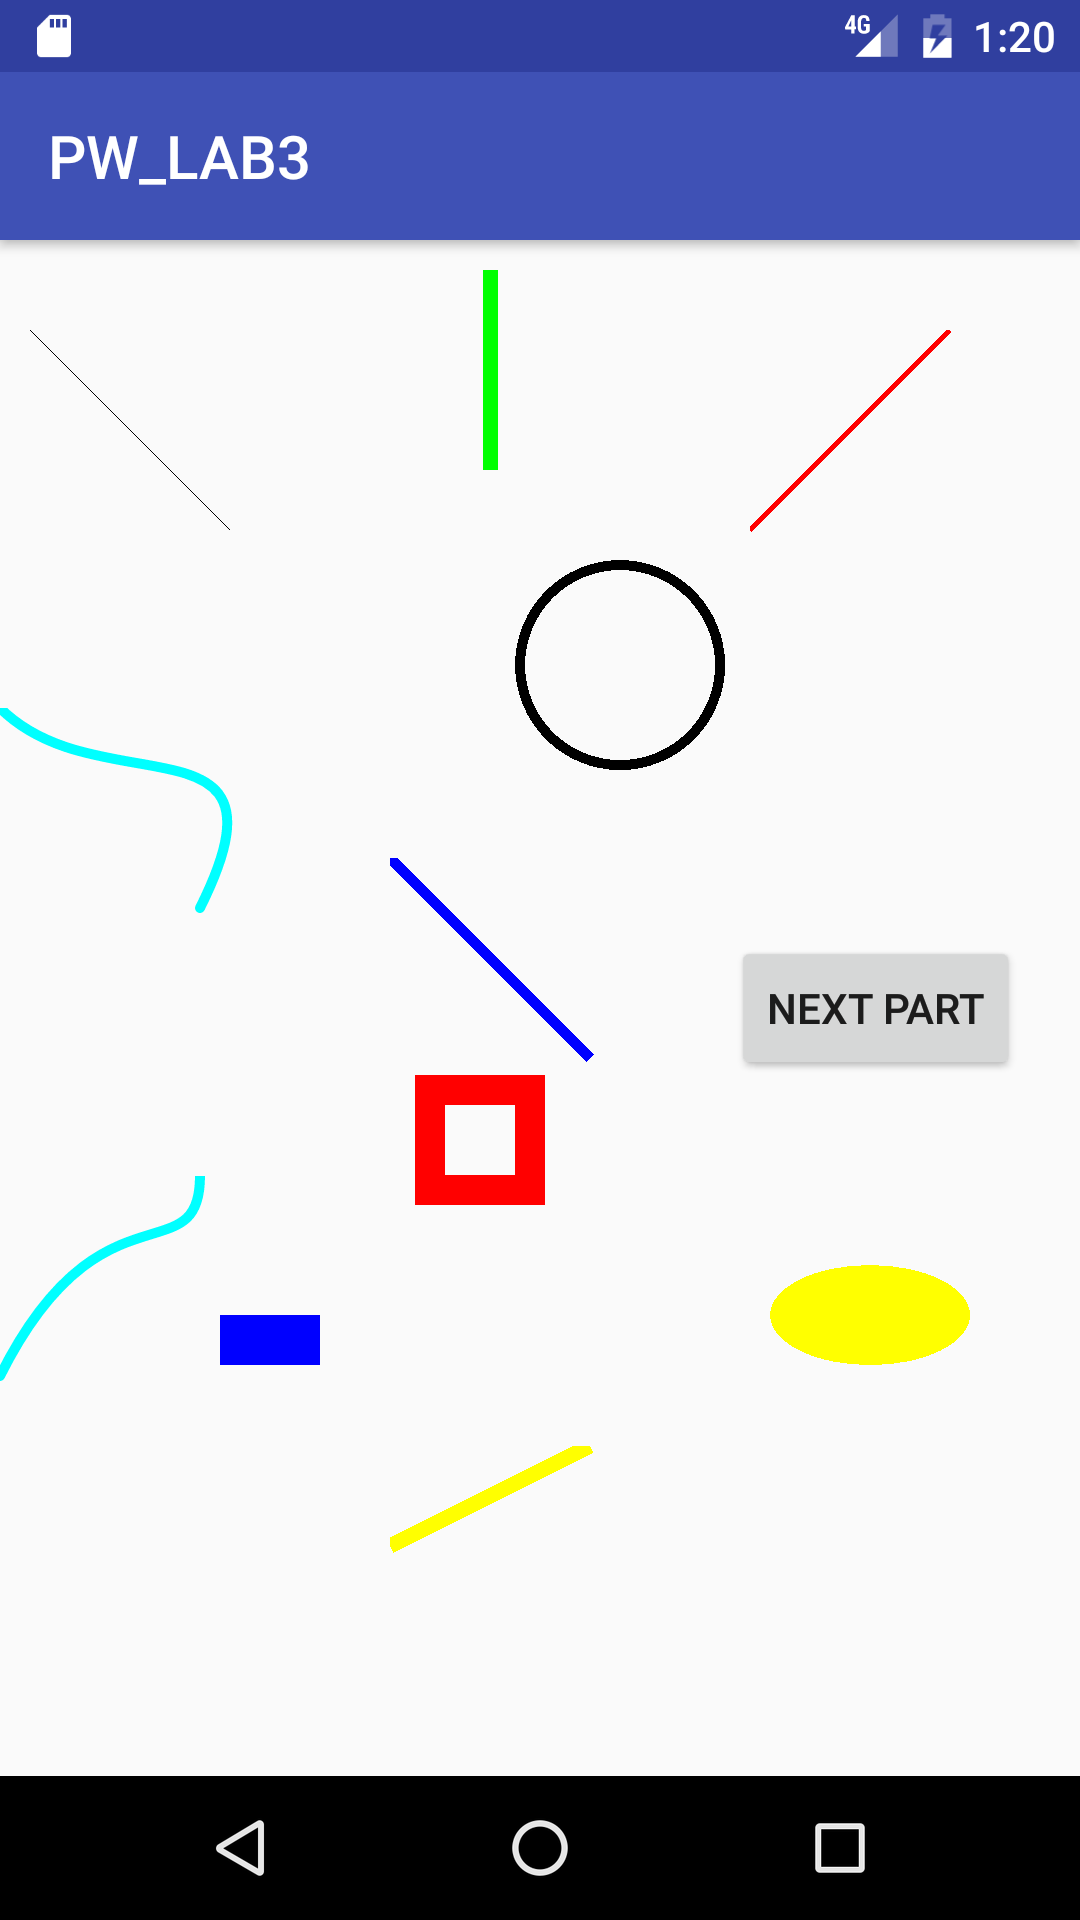
\includegraphics[scale=0.2]{screen1}
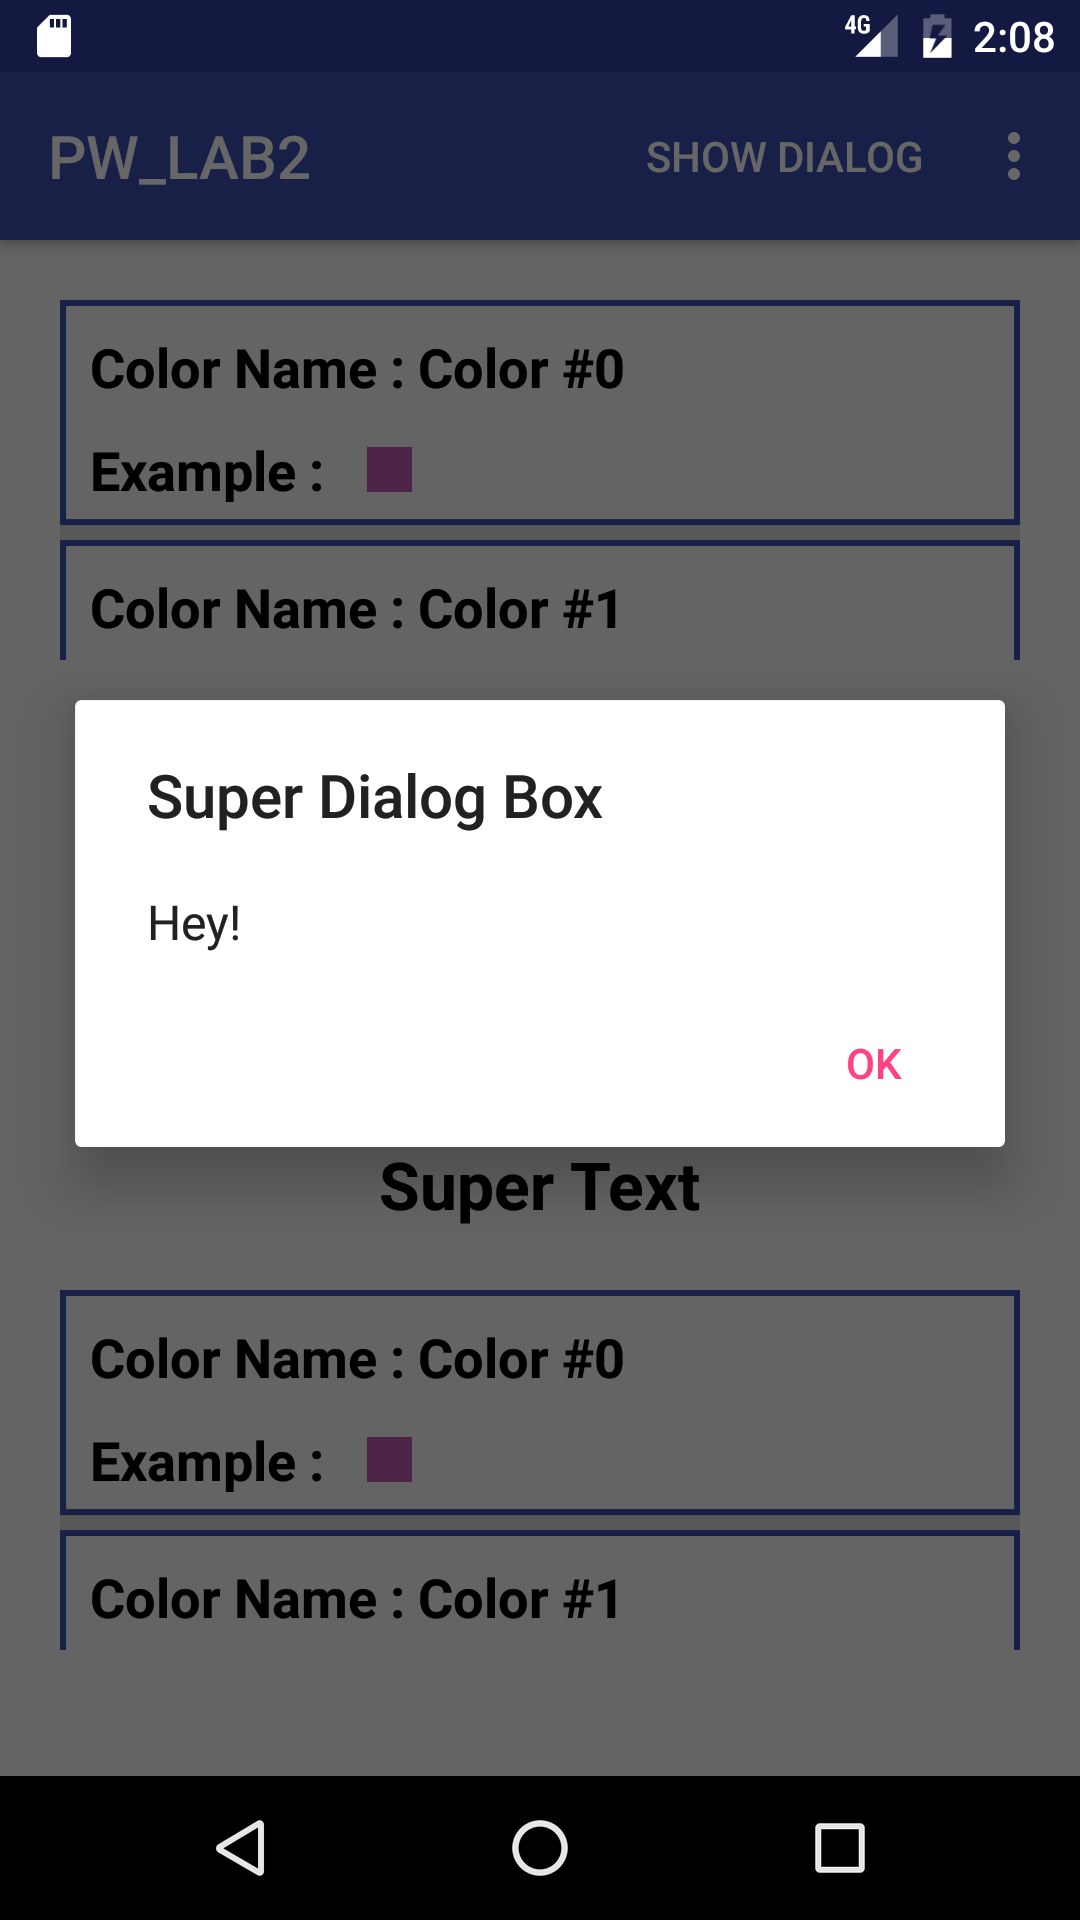
\includegraphics[scale=0.2]{screen2}

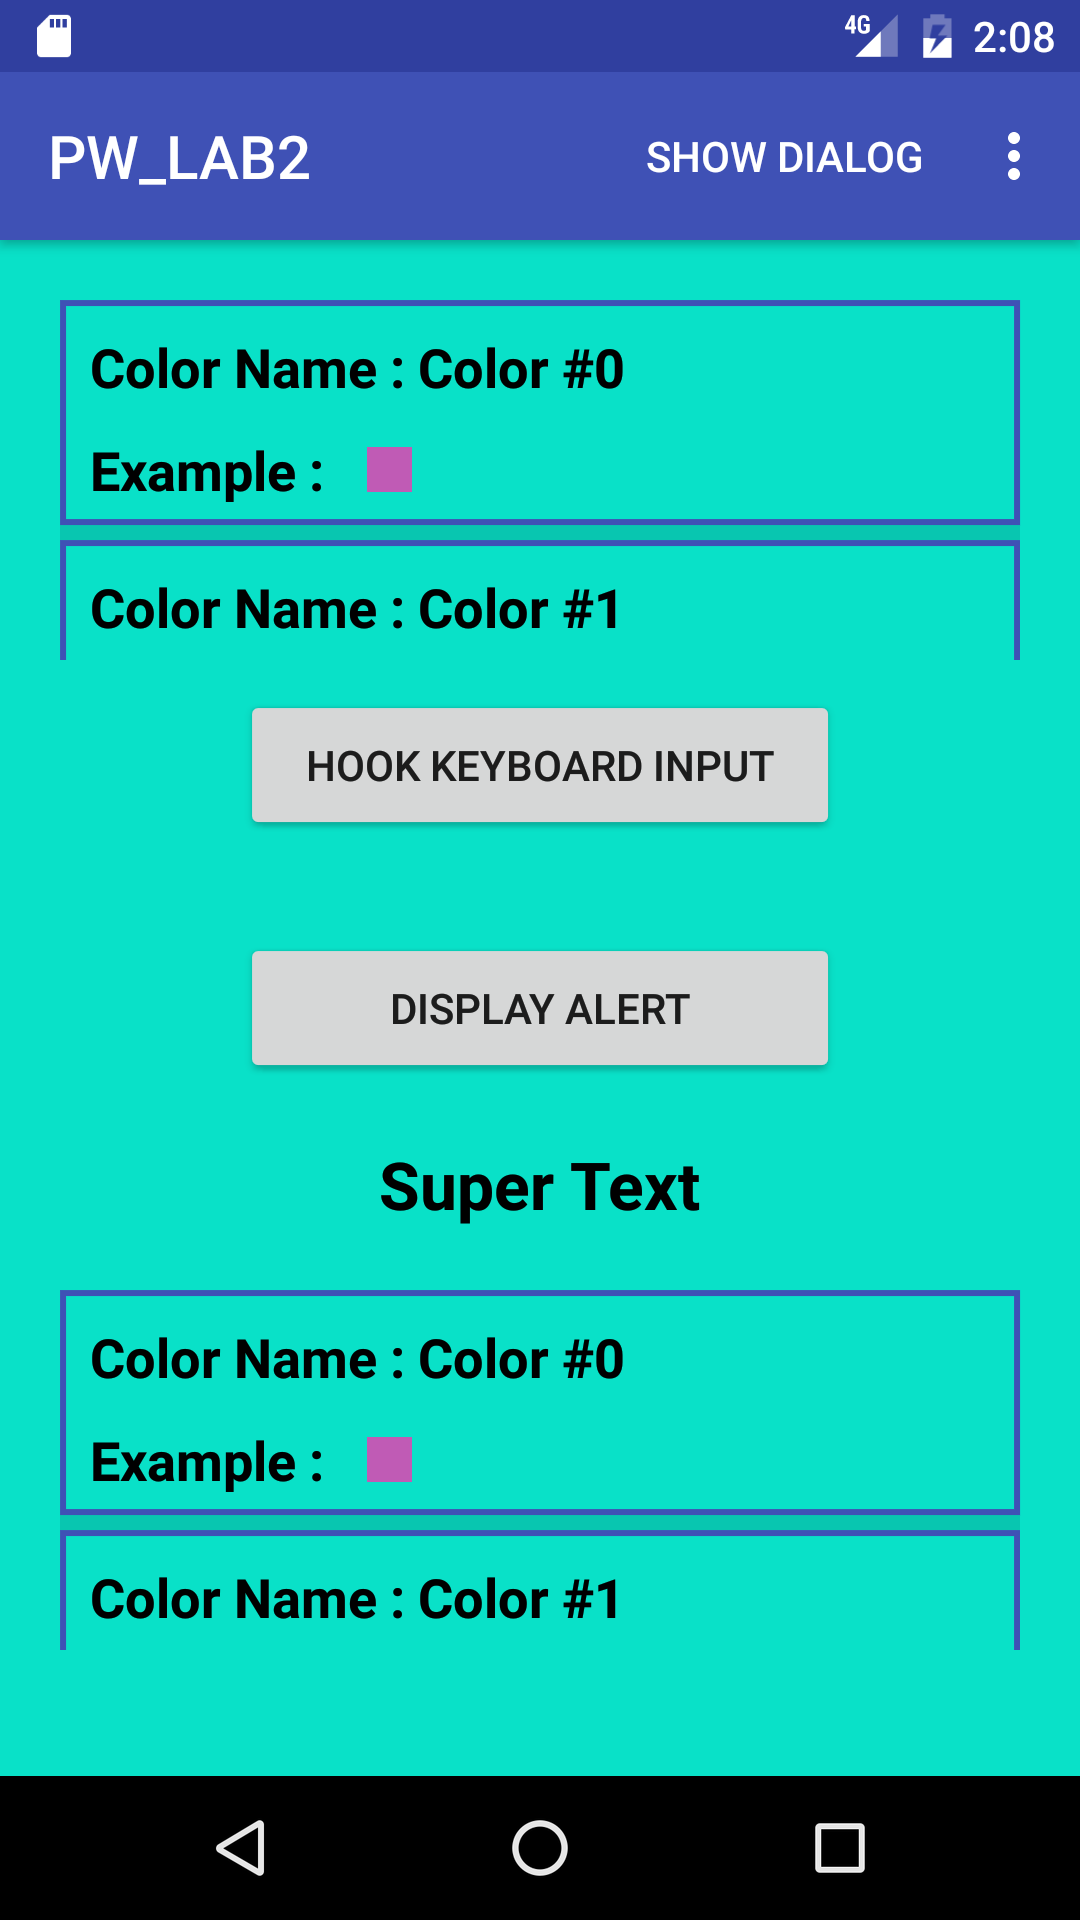
\includegraphics[scale=0.2]{screen3}
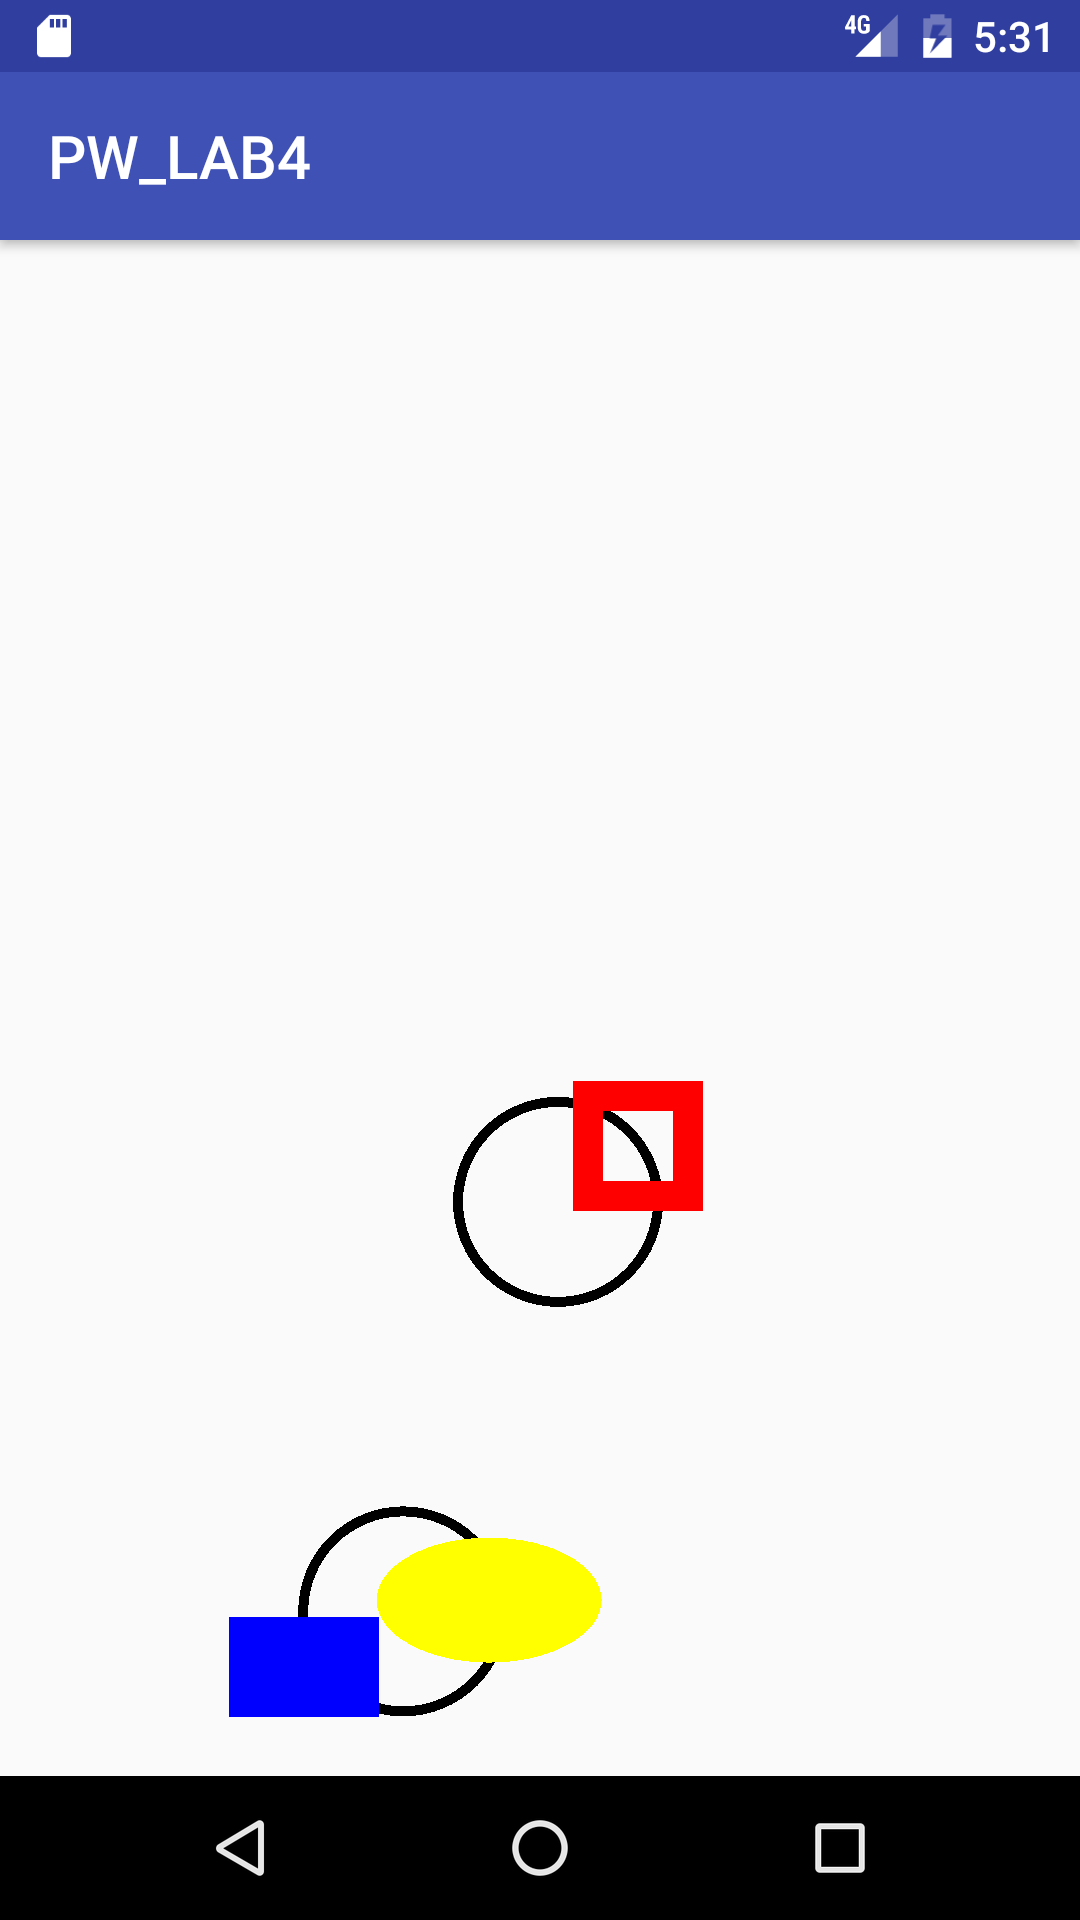
\includegraphics[scale=0.2]{screen4}

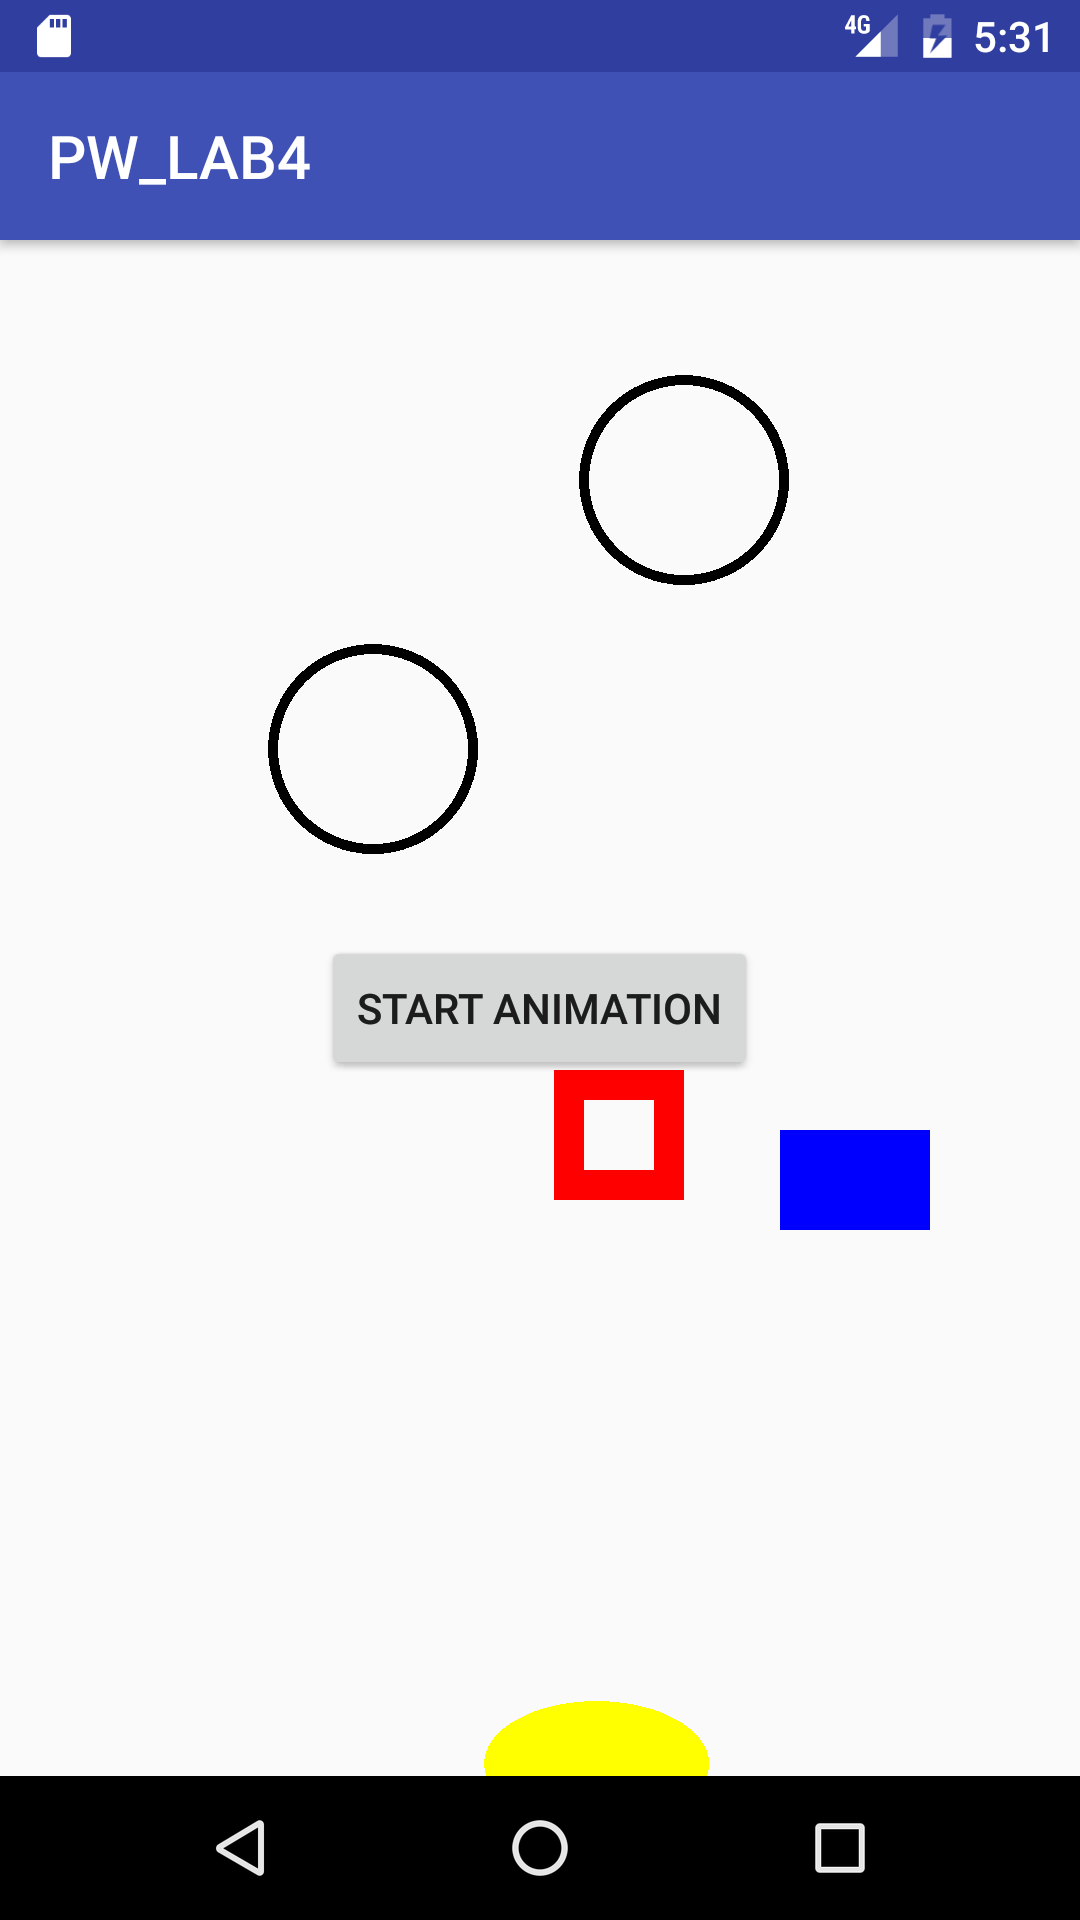
\includegraphics[scale=0.2]{screen5}

\clearpage